\section{Discussion}
The experimental investigation of the differentiator and integrator circuits' frequency response characteristics is presented in this section.
	
	\subsection{Experimental results}
		Bode plots, which graphically depict the gain and phase shift of a circuit over a range of frequencies, were employed to visualize these characteristics. \\\\
		Figures \ref{fig:differentiator_bode} and \ref{fig:integrator_bode} showcase the Bode plots of the differentiator and integrator circuits, respectively.
		To generate these plots, data was extracted from a text file containing recorded frequency values along with their corresponding circuit gain (expressed in decibels) and phase shift (in radians). 
		The dataset used for each Bode plot is also included in the Appendix (Tables \ref{tab:differentiator_data} and \ref{tab:integrator_data}). \\\\
		A logarithmic scale is employed on the x-axis to cover the range of frequencies effectively. 
		The incorporation of dual y-axes facilitates the visual comprehension of the frequency response traits exhibited by the circuits: 
		the left y-axis is dedicated to displaying gain, while the right y-axis portrays phase shift.
		To enhance clarity, data is displayed with different color markers: blue for the gain and yellow for the phase shift.

		\begin{figure}[H]
		    \centering
		    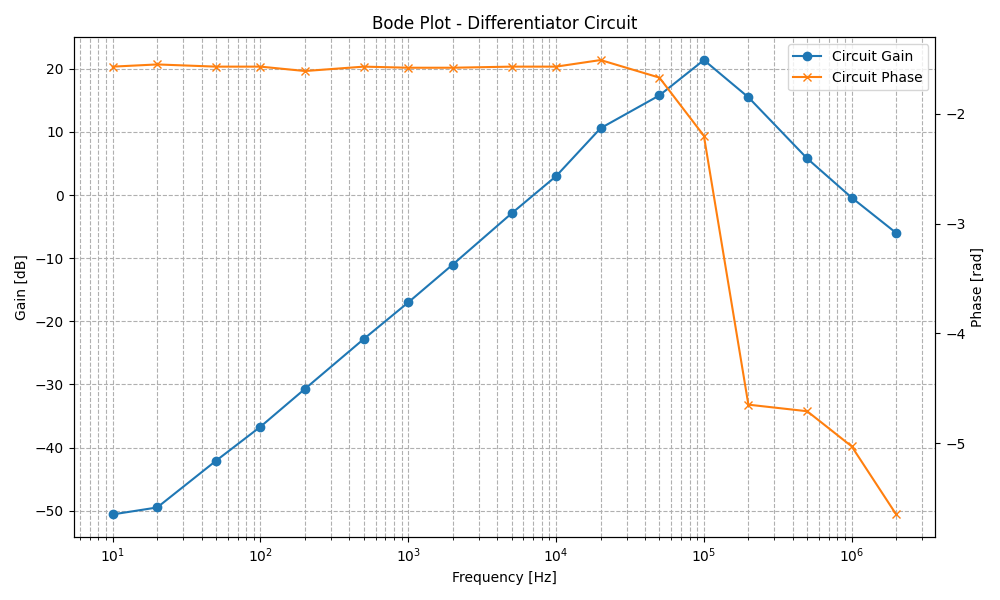
\includegraphics[width=1\textwidth]{figures/differentiator/bode_plot.png}
		    \caption{Bode plot for the differentiator circuit.}
		    \label{fig:differentiator_bode} 
		\end{figure}


		\begin{figure}[H]
		    \centering
		    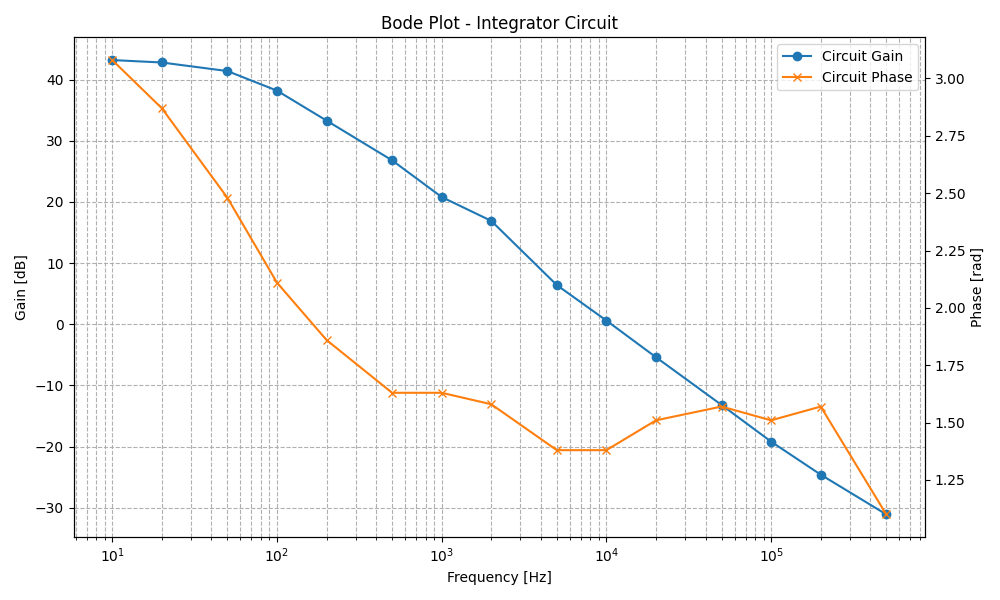
\includegraphics[width=1\textwidth]{figures/integrator/bode_plot.png}
		    \caption{Bode plot for the integrator circuit.}
		    \label{fig:integrator_bode}
		\end{figure}
	
	% comment of the Figures


	\subsection{Simulated results}
	   
		To delve deeper into the analysis of our experimental findings, the differentiator and integrator circuits were simulated using ngspice, a renowned simulation tool based on the Berkeley SPICE software. 
		This simulation process aimed to replicate the behavior of the electronic circuits under investigation. 
		The net-lists employed for simulating these circuits can be found in the Appendix for reference. \\\\
		Figures \ref{fig:differentiator_gain} and \ref{fig:differentiator_phase} provide a platform for comparing the experimental data with the corresponding simulated results for the differentiator circuit.
		Similarly, figures \ref{fig:integrator_gain} and \ref{fig:integrator_phase} present a comparative analysis between experimental and simulated data for the integrator circuit. \\
		
		\begin{figure}[H]
		    \centering
		    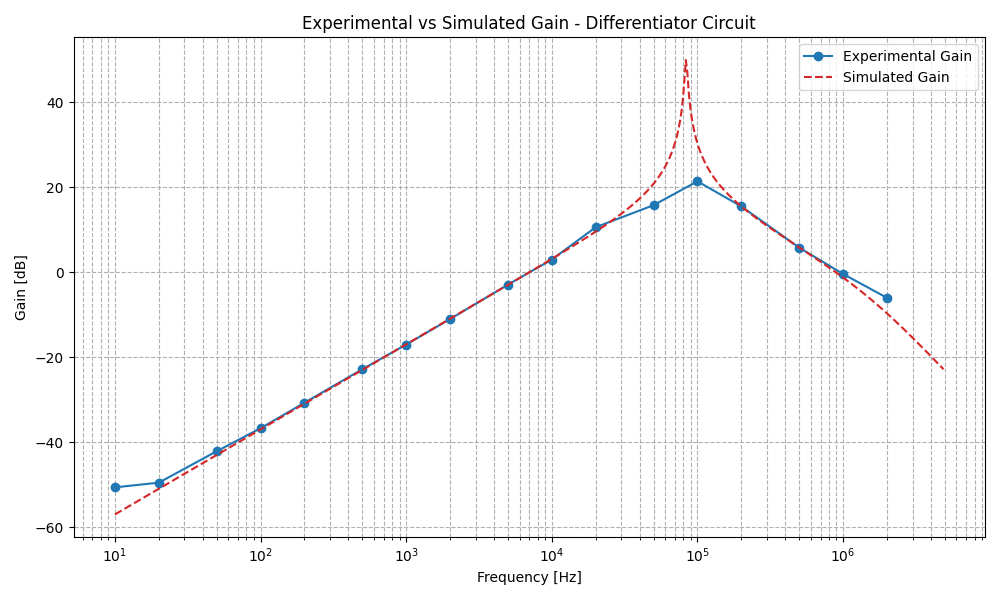
\includegraphics[width=1\textwidth]{figures/differentiator/gain_plot.png}
		    \caption{Gain comparison between experimental and simulated data for the differentiator circuit.}
		    \label{fig:differentiator_gain}
		\end{figure}

		\begin{figure}[H]
		    \centering
		    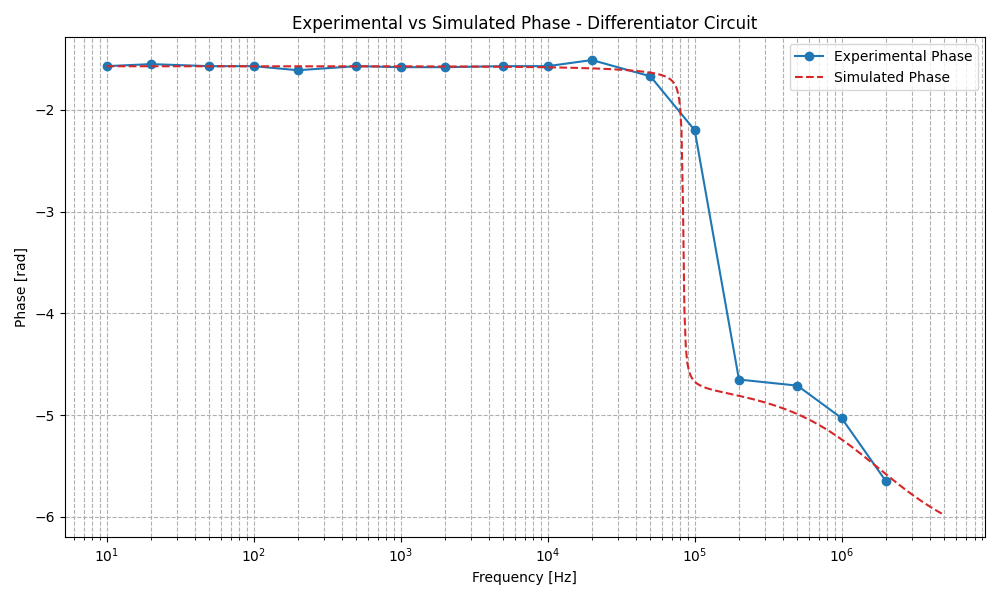
\includegraphics[width=1\textwidth]{figures/differentiator/phase_plot.png}
		    \caption{Phase comparison between experimental and simulated data for the differentiator circuit.}
		    \label{fig:differentiator_phase}
		\end{figure}

		\begin{figure}[H]
		    \centering
		    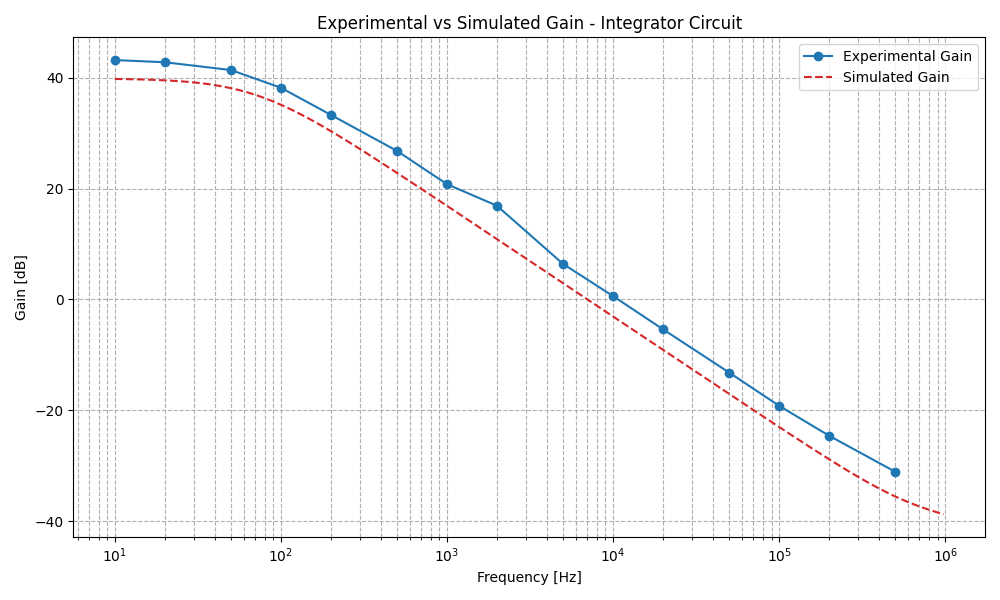
\includegraphics[width=1\textwidth]{figures/integrator/gain_plot.png}
		    \caption{Gain comparison between experimental and simulated data for the integrator circuit.}
		    \label{fig:integrator_gain}
		\end{figure}

		\begin{figure}[H]
		    \centering
		    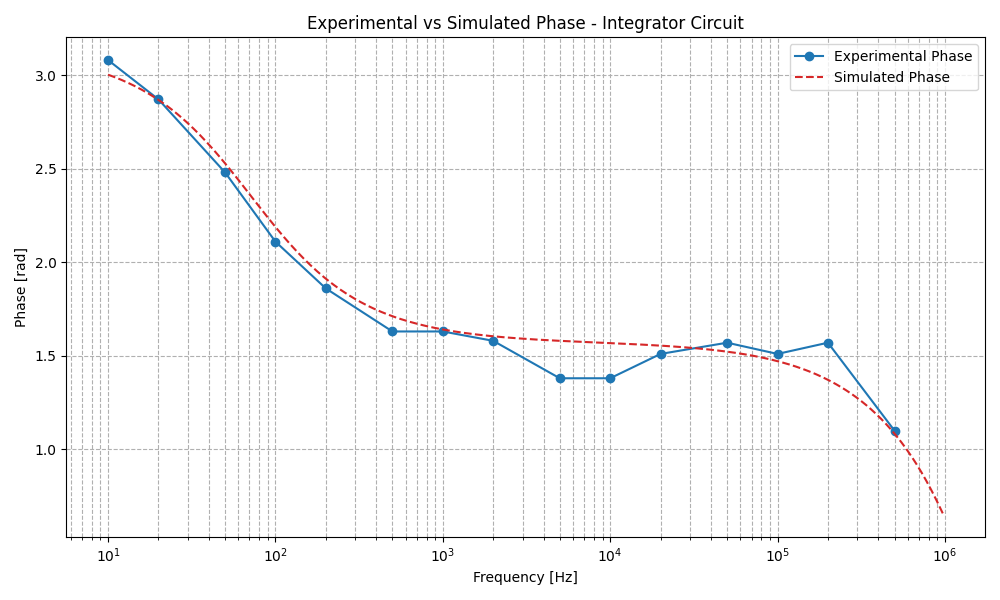
\includegraphics[width=1\textwidth]{figures/integrator/phase_plot.png}
		    \caption{Phase comparison between experimental and simulated data for the integrator circuit.}
		    \label{fig:integrator_phase}
		\end{figure} 

		The alignment between our real-world tests and simulated results demonstrates the harmony between our theoretical predictions and observed outcomes, underscoring the accuracy of our hands-on methods.
